\documentclass{beamer}
\usefonttheme[onlymath]{serif}

\usepackage{amsfonts}

% Code Block Setting
\usepackage{listings}
\lstset{language=C,
numberstyle=\footnotesize,
basicstyle=\ttfamily\footnotesize,
numbers=left,
stepnumber=1,
frame=shadowbox,
breaklines=true}

\usetheme{Warsaw}
% \usecolortheme{dove}

% Add frame number and total frame number in footline
\defbeamertemplate*{footline}{shadow theme}{%
    \leavevmode%
    \hbox{\begin{beamercolorbox}[wd=.5\paperwidth,ht=2.5ex,dp=1.125ex,leftskip=.3cm plus1fil,rightskip=.3cm]{author in head/foot}%
            \usebeamerfont{author in head/foot}\hfill\insertshortauthor
        \end{beamercolorbox}%
        \begin{beamercolorbox}[wd=.4\paperwidth,ht=2.5ex,dp=1.125ex,leftskip=.3cm,rightskip=.3cm plus1fil]{title in head/foot}%
            \usebeamerfont{title in head/foot}\insertshorttitle\hfill%
        \end{beamercolorbox}%
        \begin{beamercolorbox}[wd=.1\paperwidth,ht=2.5ex,dp=1.125ex,leftskip=.3cm,rightskip=.3cm plus1fil]{title in head/foot}%
            \hfill\insertframenumber\,/\,\inserttotalframenumber
    \end{beamercolorbox}}%
    \vskip0pt%
}

% Tikz related
\usepackage{tikz}
\usetikzlibrary{fit}
\usetikzlibrary{calc}
\usetikzlibrary{positioning}

% Number the figures
\setbeamertemplate{caption}[numbered]

% Add outline page at begining of each section
\AtBeginSection[]
{
    \begin{frame}<beamer>
        \frametitle{Outline}
        \tableofcontents[currentsection, hideallsubsections]
    \end{frame}
}

%%%%%%%%%%%%%%%%%%%%%%%%%%%%%%%%%%%%%%%%%%%%%

\title{BFS and Coloring-based Parallel Algorithms for Strongly Connected Components and Related Problems}
\author{
    George M. Slota\inst{1},\\
    Sivasankaran Rajamanickam\inst{1},\\
    Kamesh Madduri\inst{1}
}
\institute{
    \inst{1} Computer Science and Enginerring, The Pennsylvania State University
}
\date{
    \tiny{2014 IEEE 28th International Parallel and Distributed Processing Symposium}\\
    \tiny{Presented by ShiangYun Yang}
}

\begin{document}
\begin{frame}
    \titlepage
\end{frame}

\section{Introduction}

\subsection{Sparse Matrix Vector Multiplication}
\begin{frame}
    \frametitle{Definition and Propety}
	\begin{itemize}
		\item A sparse matrix is a matrix in which most of the elements 
			are zero.
		\item Sparse data is by nature more easily compressed and thus 
			require significantly less storage.
			\begin{itemize}
				\item Many formats have been proposed, such as CSR, 
					CRS, DIL, and so on.
			\end{itemize}
	\end{itemize}
\end{frame}

\subsection{CSR Format}
\begin{frame}[fragile]
	\frametitle{Compressed Row Storage}
	\begin{align*}
		A = \begin{bmatrix}
			0 & 0 & a & 0 & 0 & 0 & b & c \\
			0 & 0 & d & e & 0 & 0 & f & 0 \\
			0 & 0 & 0 & 0 & g & h & i & j \\
			k & l & 0 & 0 & m & n & o & p \\
		\end{bmatrix}
	\end{align*}
	\begin{table}[]
		\centering
		\caption{CSR format}
		\label{my-label}
		\begin{tabular}{l | c | c | c | c | c | c | c}
			\hline
		index & 0 & 1 & 2 & $\cdots$ & 12 & 13 & 14 \\ \hline
		val      & a & b & c & $\cdots$ & m & n & p  \\ \hline
		col\_ind & 2 & 6 & 7 & $\cdots$ & 4 & 5 & 7 \\ \hline
		\end{tabular}
		\\
		\begin{tabular}{l | c | c | c | c | c}
			\hline
		rowptr      & 0 & 3 & 6 & 10 & 15 \\ \hline
		\end{tabular}
	\end{table}
\end{frame}

\subsection{Serial Implementation Example}
\begin{frame}[fragile]
	\frametitle{Serial Implementation Example}
	\begin{itemize}
		\item $A_{n,m} \times x_{m,1} = y_{n,1}$
\begin{lstlisting}
for (i = 0; i < n; ++i) {
    double y0 = y[i];
    for (k = rowptr[i]; k < rowptr[i+1]; ++k)
        y0 += val[k] * x[column_index[k]];
    y[i] = y0;
}
\end{lstlisting}
	\end{itemize}
\end{frame}

\subsection{Changes of Parallel Implementation}
\begin{frame}
	\frametitle{Changes of Parallel Implementation}
	\begin{itemize}
		\item Bandwith
			\begin{itemize}
				\item the upper bound of $\text{FLOPS}\footnote{Floating-Point Operations Per Second }:\text{BYTES} = 0.25$
			\end{itemize}
		\item Load imbalance
			\begin{itemize}
				\item The non-zeros in a matrix may not be evenly distributed 
					across different rows.
				\item The matrix data have low reuse. Each non-zero element 
					is only once for computing the corresponeding dot product.
			\end{itemize}
	\end{itemize}
\end{frame}

\subsection{Executive Summary}
\begin{frame}
	\frametitle{Executive Summary}
	\begin{itemize}
		\item Improve the bandwidth by block-based compressed common
			coordinate format.
		\item Addressing the load imbalance problem by customized
			efficient segmented scan/sum.
		\item Using auto-tuning framework to explore optimization parameter 
			for different sparse matrices and different platforms.
	\end{itemize}
\end{frame}


\section{Background}

\subsection{Strongly Connected Components}
\begin{frame}
	\frametitle{Serial Algorithms}
	\begin{itemize}
		\setlength\itemsep{1em}
		\item Tarjan's Algorithm
		\item Kosaraju's Algorithm
	\end{itemize}
\end{frame}

\begin{frame}
	\frametitle{Forward-Backword Algorithm}
	\begin{itemize}
		\setlength\itemsep{1em}
		\item Let $V$ denote the set of vertices in the graph,
			$E(V)$ the set of outgoing edges, and $E'(V)$ the set
			of incoming edges.
		\item Given the graph $G(V, E(V))$, a pivot vertex $u$ is selected.
		\item A BFS search is conducted starting from $u$ to determine all 
			vertex vertices. We get \textit{descendant} set $D$ on $G(V, E(V))$ 
			and \textit{predecessor} set $P$ on $G(V, E'(V))$.
		\item The SCC $S = D \cap P$ has the pivot $u$ in it.
		\item It can be recursively called on ($D \setminus S$), 
			$(P \setminus S)$, and $(V \setminus (P \cup D))$.
	\end{itemize}
\end{frame}

\begin{frame}
	\begin{figure}
		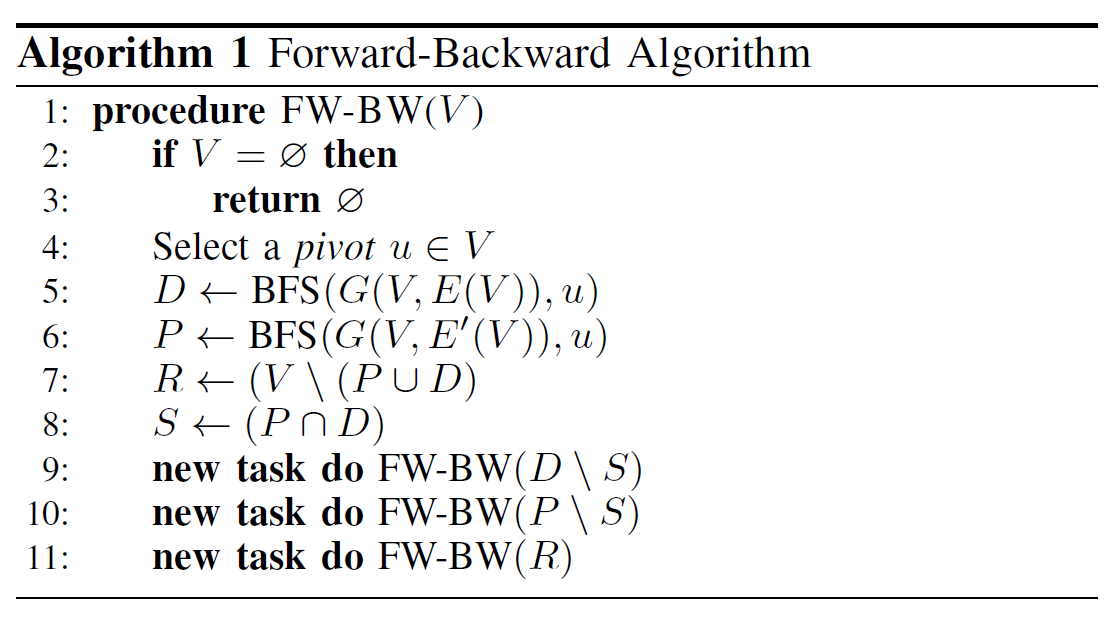
\includegraphics[scale=0.30]{figure/fig-FW-BW.png}
	\end{figure}
	\begin{itemize}
		\item For graphs with bounded constant vertex degree, 
			FW-BW is shown to perform $O(n \log n)$ expected case work.
	\end{itemize}
\end{frame}

\begin{frame}
	\frametitle{Coloring Algorithm}
	\begin{itemize}
		\setlength\itemsep{1em}
		\item This algorithm is similar to FW-BW in that it uses forward and 
			forward and backward traversals.
		\item It uses multiple pivots in the forward phase and only looks at a 
			subset of edges for each pivot in the backward phase.
		\item In a graph with a very large SCC and high diameter, the color of
			the root vertex has to be propagated to all of the verties in the
			SCC, limiting the efficiency of the color propagation step.
	\end{itemize}
\end{frame}

\begin{frame}
	\begin{figure}
		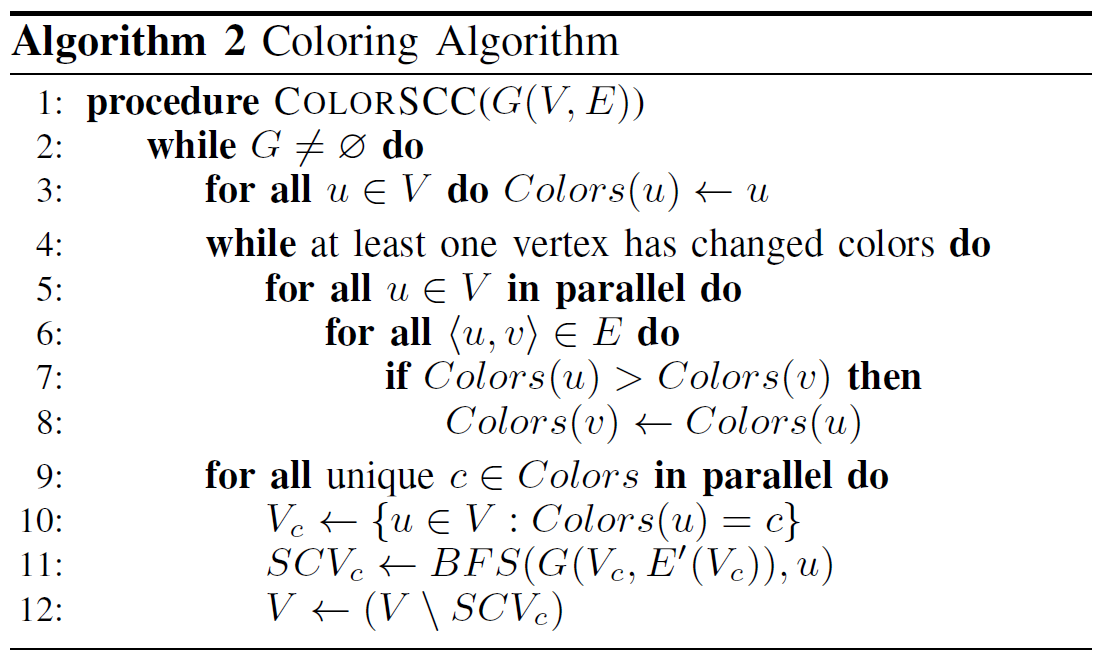
\includegraphics[scale=0.30]{figure/fig-Coloring.png}
	\end{figure}
\end{frame}

\subsection{Weakly Connected Components}
\begin{frame}
	\frametitle{Weakly Connected Components}
	There are two primary parallel methods:
	\begin{itemize}
		\setlength\itemsep{1em}
		\item Parallel BFS can be used for connected components. 
			We select new unvisted vertices as BFS roots until all vertices 
			have been visited and all connected components identified.
		\item We can use a coloring approach. Once the colors reach 
			a stable point, all vertices contained in each discrete 
			component will have the same color. \#propagation iterations 
			is bounded by $O(\log n)$.
	\end{itemize}
\end{frame}

\subsection{Biconnected Components}
\begin{frame}
	\frametitle{Biconnected Components}
	\begin{itemize}
		\setlength\itemsep{1em}
		\item The Hopcroft-Tarjan algorithm is the optimal linear-time sequential algorithm, which is based on DFS.
		\item The Tarjan-Vishkin parallel algorithm voids DFS.
	\end{itemize}
\end{frame}


\section{Multistep Method}

\subsection{Observations}
\begin{frame}
	\frametitle{FW-BW Algorithm}
	\begin{itemize}
		\setlength\itemsep{1em}
		\item[Pros] It be efficient if a graph has relatively small number 
			of large and equall-sized SCCs.
		\item[Cons] Work imbalance after the large SCC is found.
	\end{itemize}
\end{frame}

\begin{frame}
	\frametitle{Coloring Algorithm}
	\begin{itemize}
		\setlength\itemsep{1em}
		\item[Pros] It be efficient if a graph has a large number of samll
			and disconnected SCCs.
		\item[Cons] Poor initial performance on real-world graphs.
	\end{itemize}
\end{frame}

\subsection{Multistep Method}
\begin{frame}
	\frametitle{Multistep Method}
	\begin{figure}
		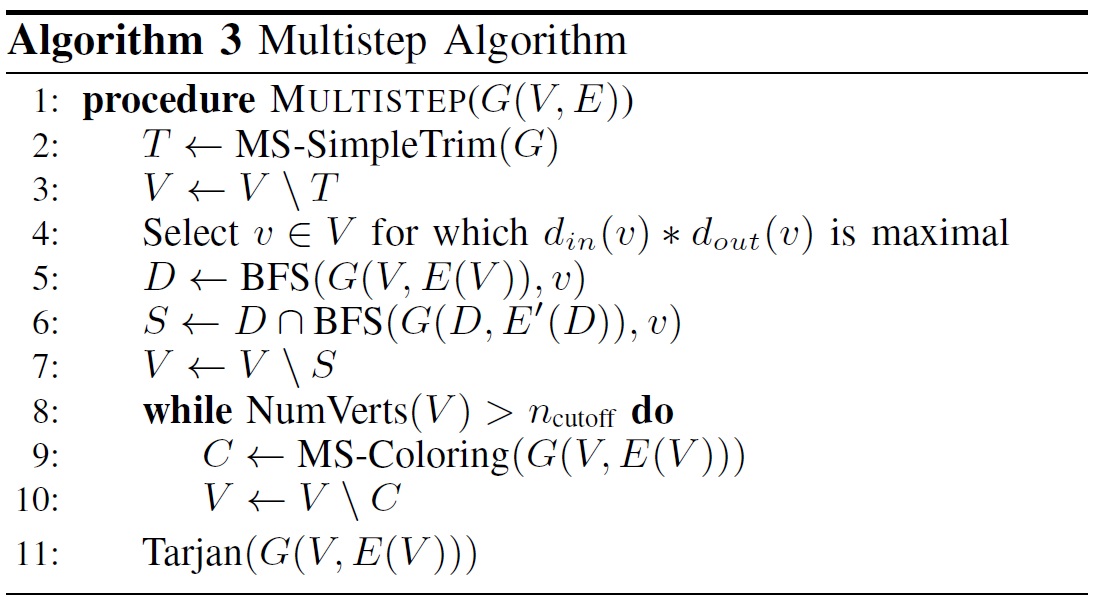
\includegraphics[scale=0.30]{figure/fig-Multistep.png}
	\end{figure}
\end{frame}

\subsection{Serial Complexity}
\begin{frame}
	\frametitle{Serial Complexity}
	\begin{itemize}
		\setlength\itemsep{0.5em}
		\item \texttt{MS-SimpleTrim(G)}
			\begin{itemize}
				\item Naive complete trimming will trim one vertex over each 
					of $n$ iterations, resulting in an upper bound of 
					$O(n^2)$ work.
				\item It uses simple trimming, or performing only a single pass
					resulting in $O(n)$ work.
			\end{itemize}
		\item \texttt{MS-Coloring(G(V,E(V)))}
			\begin{itemize}
				\item The Upper bound of naive coloring is $O(n^2)$.
				\item It uses a predefined cutoff to switch to the 
					serial algorithm.
			\end{itemize}
	\end{itemize}
	The worst case instance for Multistep will be a mostly acycle graph,
	and this would require $O(n^2)$ work.
\end{frame}

\section{Implementation}

\subsection{Implementation}
\begin{frame}
	\frametitle{Implementation}
	\begin{itemize}
		\setlength\itemsep{1em}
		\item All algorithms were implemented in C++, 
			using OpenMP for multithreading.
		\item Use the compressed sparse row (CSR) representation 
			for graph storage.
		\item To avoid modifying the graph, we have a boolean
			array termed \textit{valid} which signifies if a vertex is yet to be
			placed in an SCC.
	\end{itemize}
\end{frame}

\subsection{Trim Step}
\begin{frame}
	\frametitle{Trim Step}
	\begin{itemize}
		\setlength\itemsep{1em}
		\item It requires a single pass through all vertices to find 
			their in/out degrees, and flip their \textit{valid} boolean 
			if either degree is zero.
		\item To avoid the synchronization overhead, we maintain separate 
			queues for each thread, and combine them into the next level queue
			at the end of each iteration.
	\end{itemize}
\end{frame}

\subsection{Breath-First Search}
\begin{frame}
	\frametitle{Breath-First Search}
	\begin{itemize}
		\setlength\itemsep{1em}
		\item Using thread-local queues instead of a shared queue avoids the 
			synchronization overhead of insertions.
		\item A boolean \textit{visited} array outerperforms a bitmap.
		\item In this \textit{direction-optimizing} approach to BFS, all
			unvisited vertices attempt to find a parent that is in the 
			frontier, instead of the typical way of inspecting adjacencies of
			frontier vertices.
	\end{itemize}
\end{frame}

\subsection{Coloring}
\begin{frame}
	\frametitle{Coloring}
	\begin{itemize}
		\item Place the parent in queue to avoid explicit locking.
	\end{itemize}
	\begin{figure}
		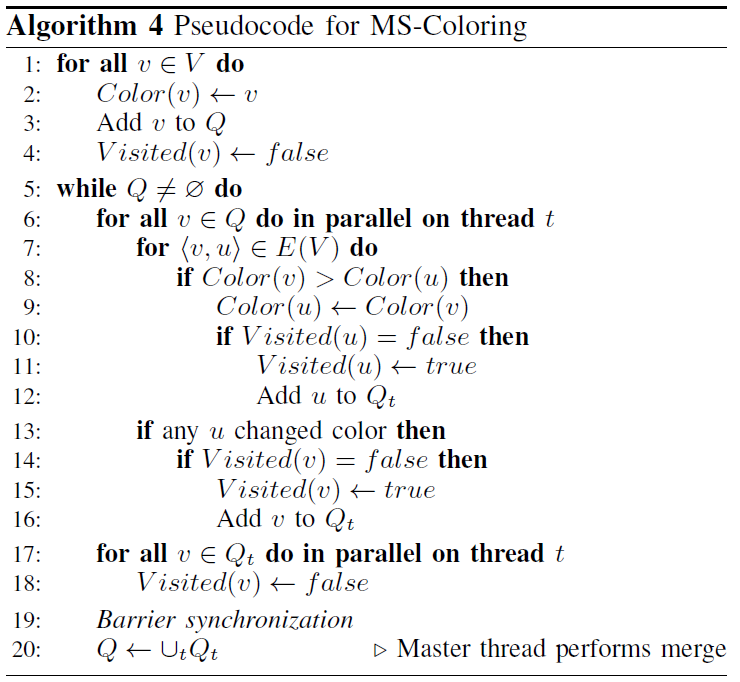
\includegraphics[scale=0.30]{figure/fig-MS-coloring.png}
	\end{figure}
\end{frame}

\subsection{BiCC Decomposition}
\begin{frame}
	\frametitle{BiCC Decomposition}
	\begin{itemize}
		\setlength\itemsep{1em}
		\item A new parallel approach for BiCC decomposition by identifying 
			articulation vertices in graph.
		\item An articulation vertex $u$ can be identified by the fact that it 
			has at least one child vertex that does not have a simple path in
			$G(V \setminus \{u\}, E(V \setminus \{u\})))$ to another vertex with 
			the same BFS level as $u$.
	\end{itemize}
\end{frame}

\begin{frame}
	\begin{figure}
		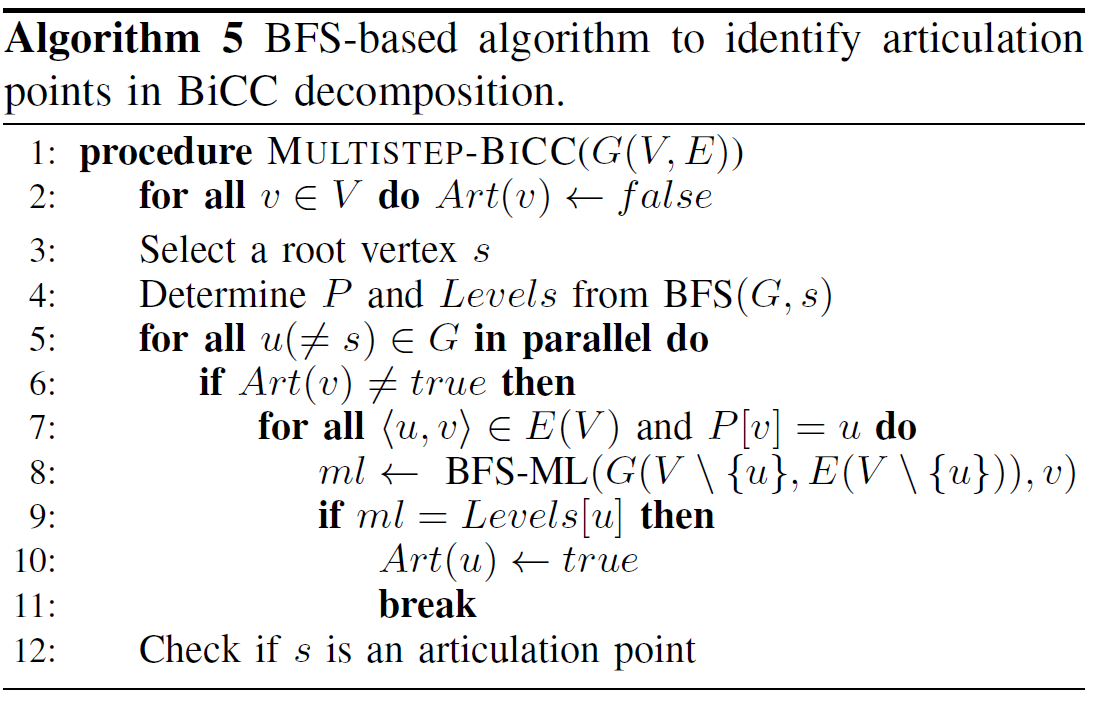
\includegraphics[scale=0.25]{figure/fig-BBC-BFS-based.png}
	\end{figure}
\end{frame}
\section{Experiment}

\subsection{Configuration}
\begin{frame}
    \frametitle{Configuration}
    \begin{itemize}
    	\item Four versions
		    \begin{itemize}
				\item \textit{LOOPDP}: optimized looping code with padding
					to mitigate set-associativity problem.
				\item \textit{CO}: unoptimized CORDAC.
				\item \textit{CO\_Opt}: optimized CORDAC + copy-optimization.
				\item \textit{COZ}: \textit{CO\_Opt} + \textit{ZM\_RM} 
					layout for data storage.
			\end{itemize}
		\item Base-case size of $64 \times 64$ for parenthesis, gap and protein 
			folding and $128 \times 128$ for FW-APSP.
	\end{itemize}
\end{frame}

\subsection{Platforms}
\begin{frame}
    \frametitle{Platforms}
    \begin{figure}
		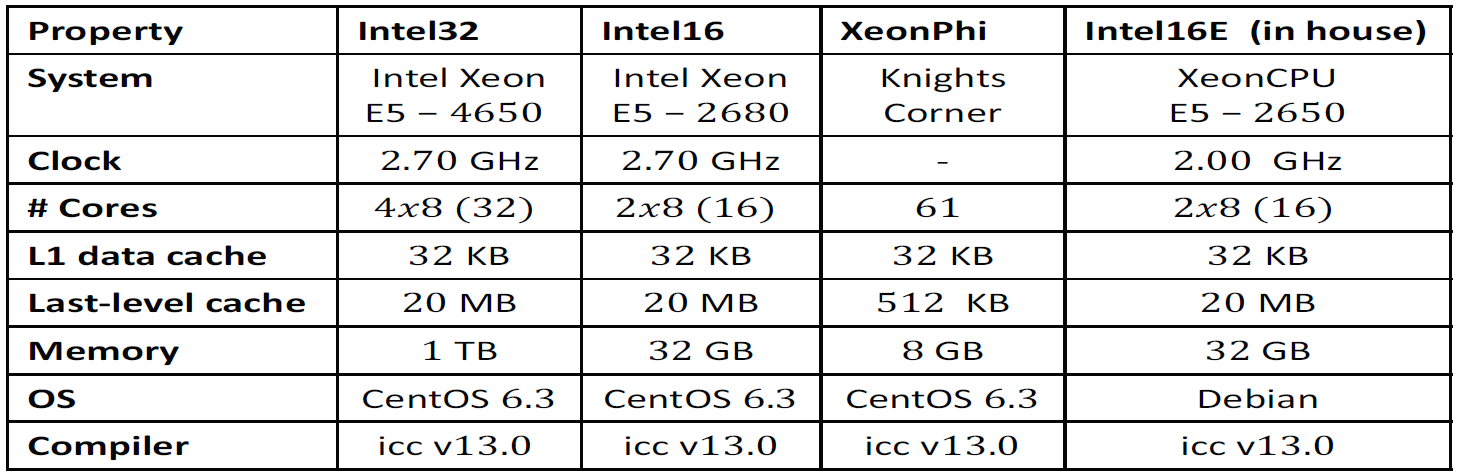
\includegraphics[scale=0.3]{figure/fig-platforms.png}
	\end{figure}
\end{frame}

\subsection{Shared-Memory Machine}
\begin{frame}
    \frametitle{Performance on Shared-Memory Machine}
    \begin{itemize}
    	\item For parenthesization problem, hybrid CPU + 
    		Xeon Phi version runs $395\times$ for $n = 32768$.
    	\item Explicit vectorization contributed up to $5\times$ speedup
    		over auto-vectorized code.
    	\item CORDAC algorithms consume $4$ -- $30\times$ less energy.
    \end{itemize}
\end{frame}

\begin{frame}
    \begin{figure}
		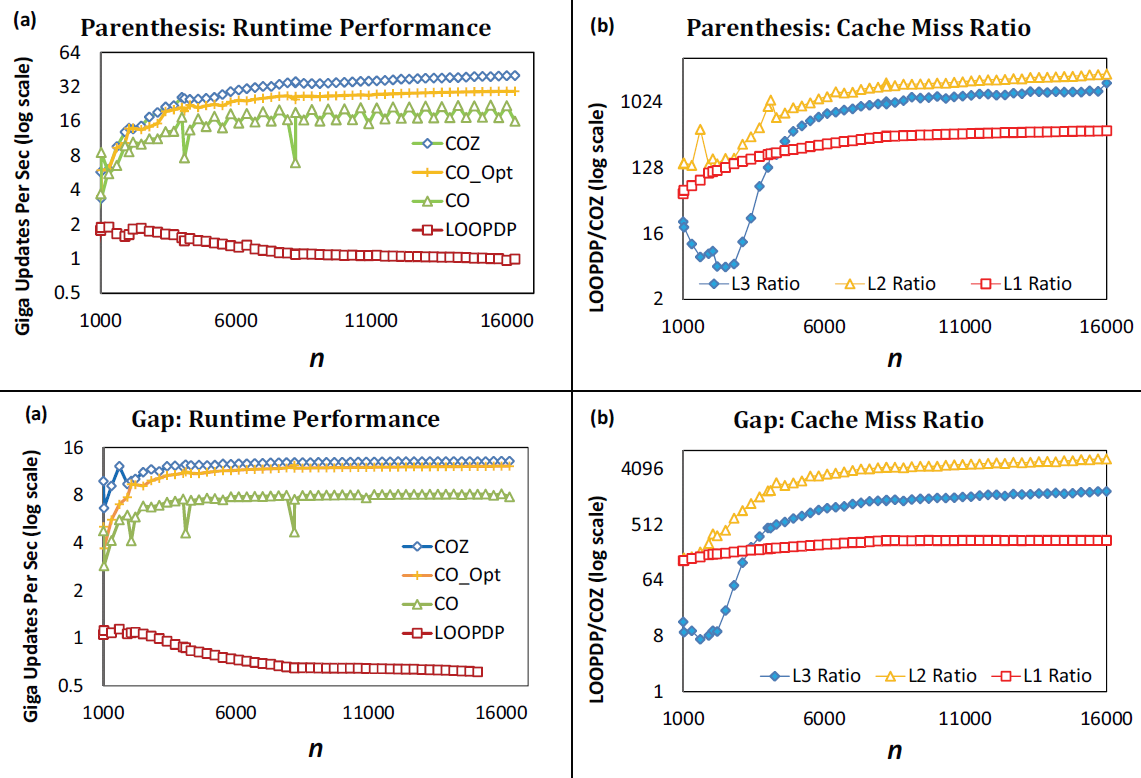
\includegraphics[scale=0.3]{figure/fig-shared-machine-1.png}
	\end{figure}
	\footnote{Performance on Intel 16: Intel Xeon E5-2680}
\end{frame}

\begin{frame}
    \begin{figure}
		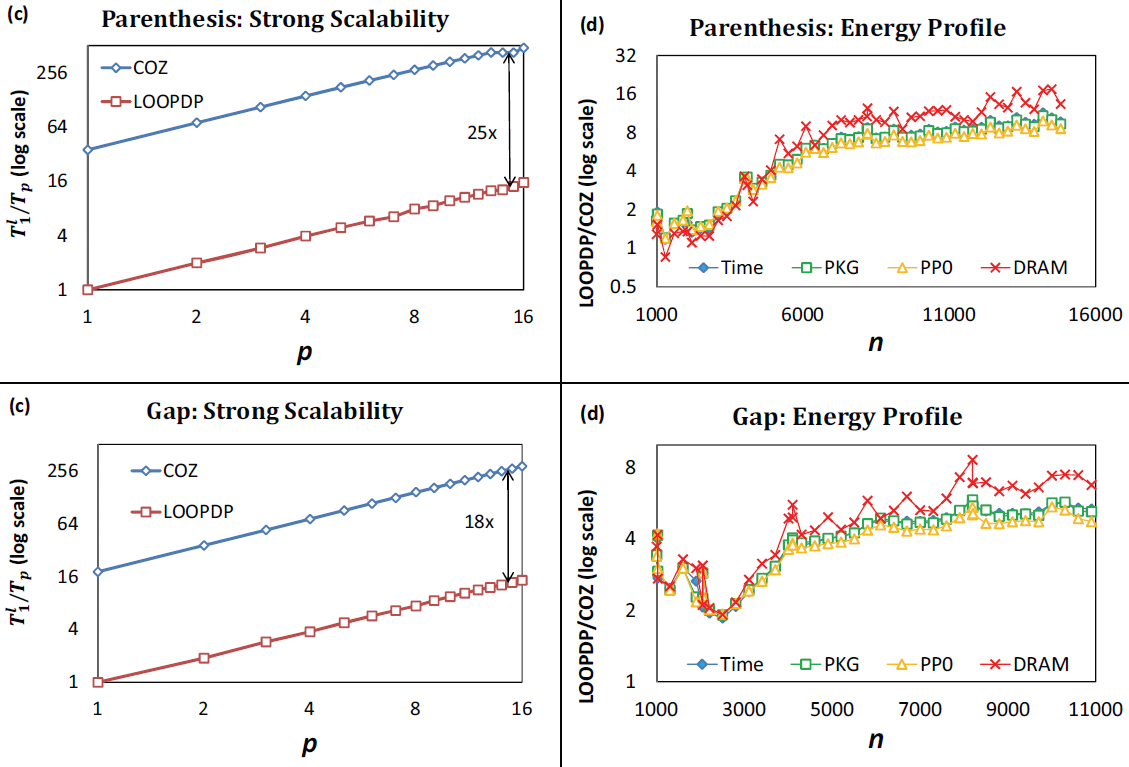
\includegraphics[scale=0.3]{figure/fig-shared-machine-2.png}
	\end{figure}
	\footnote{Performance on Intel 16: Intel Xeon E5-2680}
\end{frame}


\end{document}
